\section{Operações de inserção}

\begin{frame}[fragile]{Anexar ao final do vetor}

    \begin{itemize}
        \item Dentre as duas operações de inserção definidas, a operação
        \rawcode{push\_back()} é a que tem menor complexidade assintótica

        \item Se ainda houver espaço disponível no vetor, basta inserir o valor
        indicado na posição correspondente e atualizar o valor do campo \rawcode{size}

        \item Se o vetor estiver cheio (isto é, se o tamanho for igual a capacidade), há 
        duas estratégias possível

        \item A mais simples, e que mantém o pior caso em $O(1)$, é retornar um código de erro

        \item A segunda seria ampliar a capacidade do vetor para comportar novos elementos

        \item A complexidade do pior caso seria então $O(N)$, mas o custo amortizado seria
        $O(1)$
    \end{itemize}

\end{frame}

\begin{frame}[fragile]{Visualização da inserção}

    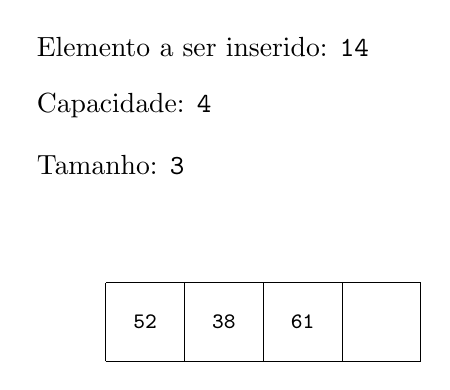
\begin{tikzpicture}
        \node[anchor=west] at (0, 4) {Elemento a ser inserido: \texttt{14}};
        \node[anchor=west] at (0, 3.25) {Capacidade: \texttt{4}};
        \node[anchor=west] at (0, 2.5) {Tamanho: \texttt{3}};
        \draw (1,0) grid (5,1);

        \node at (1.5,0.5) {\footnotesize \texttt{52}};
        \node at (2.5,0.5) {\footnotesize \texttt{38}};
        \node at (3.5,0.5) {\footnotesize \texttt{61}};
    \end{tikzpicture}

\end{frame}

\begin{frame}[fragile]{Visualização da inserção}

    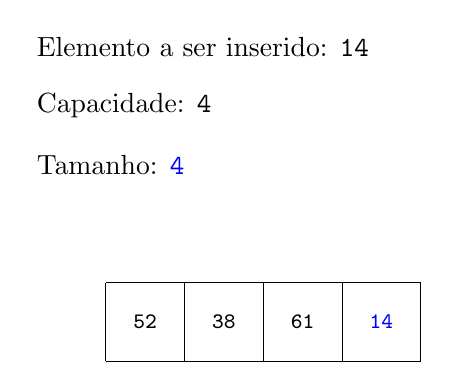
\begin{tikzpicture}
        \node[anchor=west] at (0, 4) {Elemento a ser inserido: \texttt{14}};
        \node[anchor=west] at (0, 3.25) {Capacidade: \texttt{4}};
        \node[anchor=west] at (0, 2.5) {Tamanho: \texttt{\textcolor{blue}{4}}};
        \draw (1,0) grid (5,1);

        \node at (1.5,0.5) {\footnotesize \texttt{52}};
        \node at (2.5,0.5) {\footnotesize \texttt{38}};
        \node at (3.5,0.5) {\footnotesize \texttt{61}};
        \node at (4.5,0.5) {\footnotesize \texttt{\textcolor{blue}{14}}};
    \end{tikzpicture}

\end{frame}

\begin{frame}[fragile]{Visualização da inserção}

    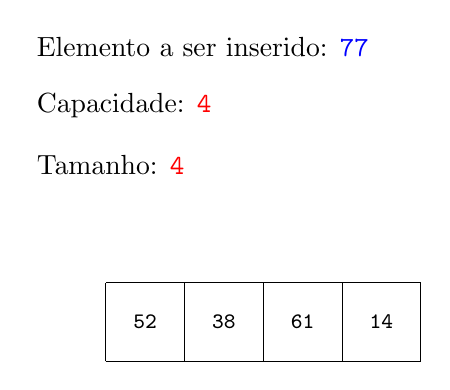
\begin{tikzpicture}
        \node[anchor=west] at (0, 4) {Elemento a ser inserido: \texttt{\textcolor{blue}{77}}};
        \node[anchor=west] at (0, 3.25) {Capacidade: \texttt{\textcolor{red}{4}}};
        \node[anchor=west] at (0, 2.5) {Tamanho: \texttt{\textcolor{red}{4}}};
        \draw (1,0) grid (5,1);

        \node at (1.5,0.5) {\footnotesize \texttt{52}};
        \node at (2.5,0.5) {\footnotesize \texttt{38}};
        \node at (3.5,0.5) {\footnotesize \texttt{61}};
        \node at (4.5,0.5) {\footnotesize \texttt{14}};
    \end{tikzpicture}

\end{frame}

\begin{frame}[fragile]{Visualização da inserção}

    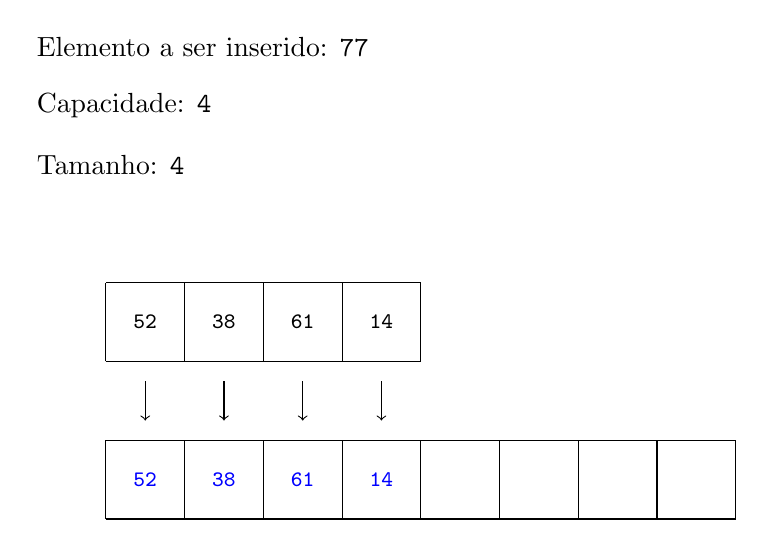
\begin{tikzpicture}
        \node[anchor=west] at (0, 4) {Elemento a ser inserido: \texttt{\textcolor{black}{77}}};
        \node[anchor=west] at (0, 3.25) {Capacidade: \texttt{\textcolor{black}{4}}};
        \node[anchor=west] at (0, 2.5) {Tamanho: \texttt{\textcolor{black}{4}}};
        \draw (1,0) grid (5,1);
        \draw (1,-2) grid (9,-1);

        \node at (1.5,0.5) {\footnotesize \texttt{52}};
        \node at (2.5,0.5) {\footnotesize \texttt{38}};
        \node at (3.5,0.5) {\footnotesize \texttt{61}};
        \node at (4.5,0.5) {\footnotesize \texttt{14}};

        \draw [->] (1.5,-0.25) -- (1.5,-0.75);
        \draw [->] (2.5,-0.25) -- (2.5,-0.75);
        \draw [->] (3.5,-0.25) -- (3.5,-0.75);
        \draw [->] (4.5,-0.25) -- (4.5,-0.75);

        \node at (1.5,-1.5) {\footnotesize \texttt{\textcolor{blue}{52}}};
        \node at (2.5,-1.5) {\footnotesize \texttt{\textcolor{blue}{38}}};
        \node at (3.5,-1.5) {\footnotesize \texttt{\textcolor{blue}{61}}};
        \node at (4.5,-1.5) {\footnotesize \texttt{\textcolor{blue}{14}}};
    \end{tikzpicture}

\end{frame}

\begin{frame}[fragile]{Visualização da inserção}

    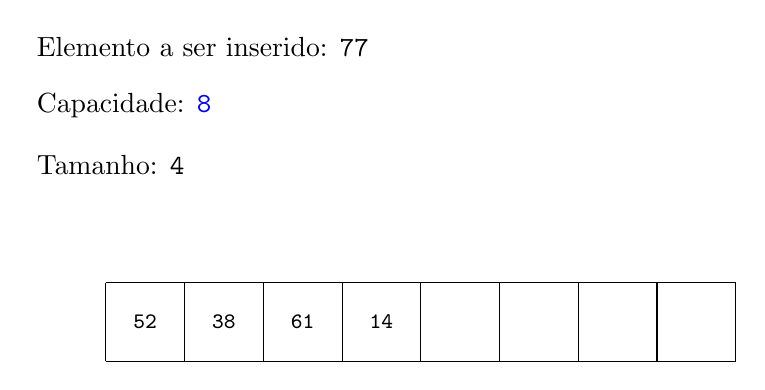
\begin{tikzpicture}
        \node[anchor=west] at (0, 4) {Elemento a ser inserido: \texttt{\textcolor{black}{77}}};
        \node[anchor=west] at (0, 3.25) {Capacidade: \texttt{\textcolor{blue}{8}}};
        \node[anchor=west] at (0, 2.5) {Tamanho: \texttt{\textcolor{black}{4}}};
        \draw (1,0) grid (9,1);

        \node at (1.5,0.5) {\footnotesize \texttt{52}};
        \node at (2.5,0.5) {\footnotesize \texttt{38}};
        \node at (3.5,0.5) {\footnotesize \texttt{61}};
        \node at (4.5,0.5) {\footnotesize \texttt{14}};
    \end{tikzpicture}

\end{frame}

\begin{frame}[fragile]{Visualização da inserção}

    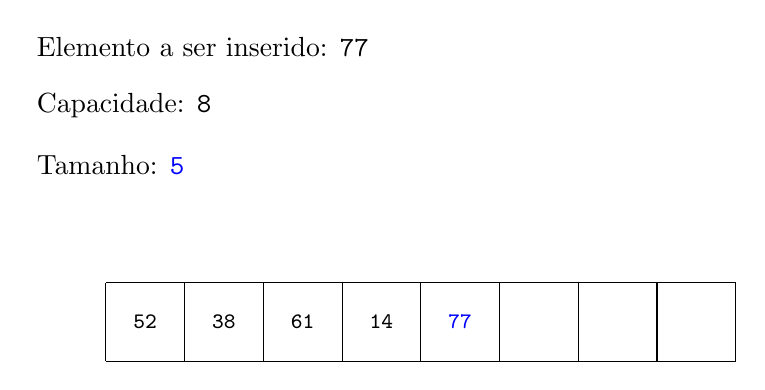
\begin{tikzpicture}
        \node[anchor=west] at (0, 4) {Elemento a ser inserido: \texttt{\textcolor{black}{77}}};
        \node[anchor=west] at (0, 3.25) {Capacidade: \texttt{\textcolor{black}{8}}};
        \node[anchor=west] at (0, 2.5) {Tamanho: \texttt{\textcolor{blue}{5}}};
        \draw (1,0) grid (9,1);

        \node at (1.5,0.5) {\footnotesize \texttt{52}};
        \node at (2.5,0.5) {\footnotesize \texttt{38}};
        \node at (3.5,0.5) {\footnotesize \texttt{61}};
        \node at (4.5,0.5) {\footnotesize \texttt{14}};
        \node at (5.5,0.5) {\footnotesize \texttt{\textcolor{blue}{77}}};
    \end{tikzpicture}

\end{frame}

\begin{frame}[fragile]{Implementação da função \rawcode{push\_back()}}
    \inputsnippet{c}{64}{84}{vector_adt.c}
\end{frame}

\begin{frame}[fragile]{Inserção em posição arbitrária}

    \begin{itemize}
        \item A inserção em uma posição arbitrária \rawcode{i} do vetor em complexidade $O(N)$

        \item Assim como a inserção ao final do vetor, pode ser necessário ampliar a capacidade
        do vetor caso este esteja cheio

        \item Todos os elementos, a partir da posição \rawcode{i} em diante, devem ser deslocados
        uma posição para a direita

        \item Uma vez realizado o deslocamento, o valor indicado pode ser escrito na posição
        \rawcode{i}

        \item O tamanho do vetor também deve ser atualizado
    \end{itemize}

\end{frame}

\begin{frame}[fragile]{Visualização da inserção em posição arbitrária}

    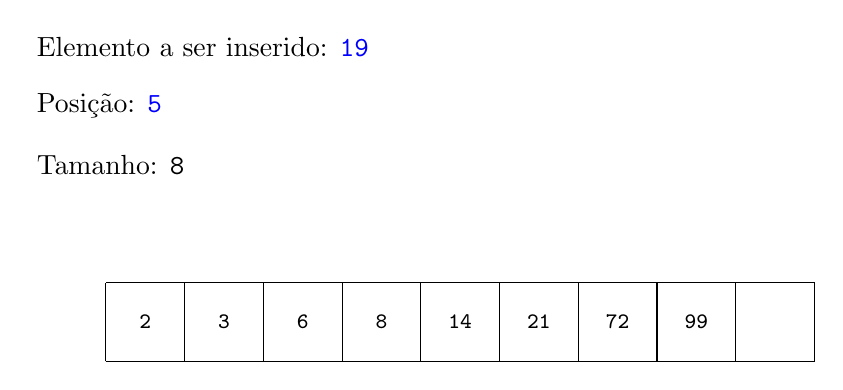
\begin{tikzpicture}
        \node[anchor=west] at (0, 4) {Elemento a ser inserido: \texttt{\textcolor{blue}{19}}};
        \node[anchor=west] at (0, 3.25) {Posição: \texttt{\textcolor{blue}{5}}};
        \node[anchor=west] at (0, 2.5) {Tamanho: \texttt{\textcolor{black}{8}}};
        \draw (1,0) grid (10,1);

        \node at (1.5,0.5) {\footnotesize \texttt{2}};
        \node at (2.5,0.5) {\footnotesize \texttt{3}};
        \node at (3.5,0.5) {\footnotesize \texttt{6}};
        \node at (4.5,0.5) {\footnotesize \texttt{8}};
        \node at (5.5,0.5) {\footnotesize \texttt{14}};
        \node at (6.5,0.5) {\footnotesize \texttt{21}};
        \node at (7.5,0.5) {\footnotesize \texttt{72}};
        \node at (8.5,0.5) {\footnotesize \texttt{99}};
    \end{tikzpicture}

\end{frame}

\begin{frame}[fragile]{Visualização da inserção em posição arbitrária}

    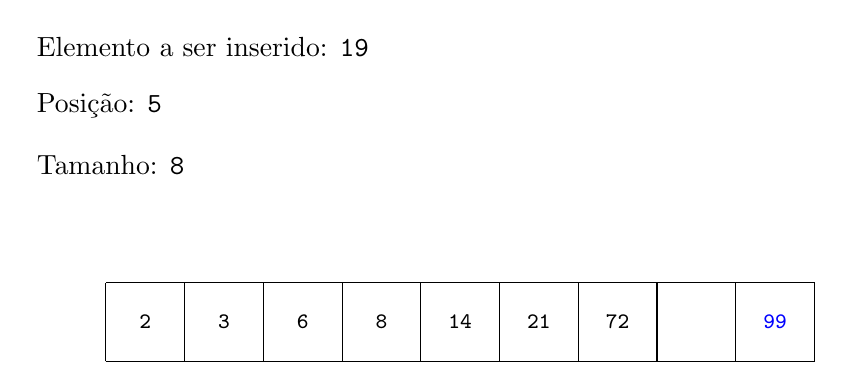
\begin{tikzpicture}
        \node[anchor=west] at (0, 4) {Elemento a ser inserido: \texttt{\textcolor{black}{19}}};
        \node[anchor=west] at (0, 3.25) {Posição: \texttt{\textcolor{black}{5}}};
        \node[anchor=west] at (0, 2.5) {Tamanho: \texttt{\textcolor{black}{8}}};
        \draw (1,0) grid (10,1);

        \node at (1.5,0.5) {\footnotesize \texttt{2}};
        \node at (2.5,0.5) {\footnotesize \texttt{3}};
        \node at (3.5,0.5) {\footnotesize \texttt{6}};
        \node at (4.5,0.5) {\footnotesize \texttt{8}};
        \node at (5.5,0.5) {\footnotesize \texttt{14}};
        \node at (6.5,0.5) {\footnotesize \texttt{21}};
        \node at (7.5,0.5) {\footnotesize \texttt{72}};
        \node at (8.5,0.5) {\footnotesize \texttt{}};
        \node at (9.5,0.5) {\footnotesize \texttt{\textcolor{blue}{99}}};
    \end{tikzpicture}

\end{frame}

\begin{frame}[fragile]{Visualização da inserção em posição arbitrária}

    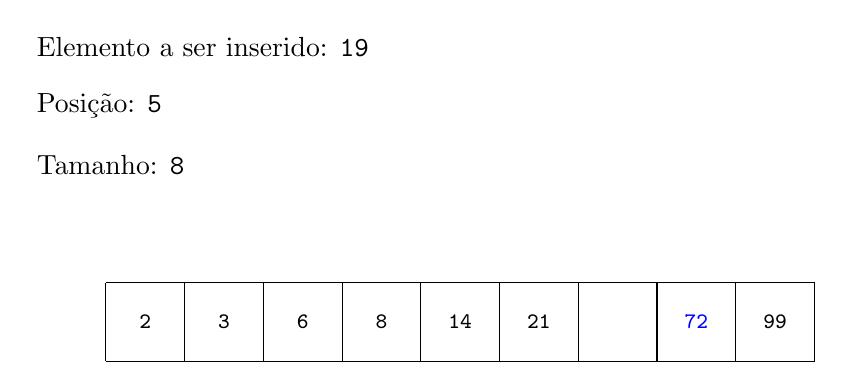
\begin{tikzpicture}
        \node[anchor=west] at (0, 4) {Elemento a ser inserido: \texttt{\textcolor{black}{19}}};
        \node[anchor=west] at (0, 3.25) {Posição: \texttt{\textcolor{black}{5}}};
        \node[anchor=west] at (0, 2.5) {Tamanho: \texttt{\textcolor{black}{8}}};
        \draw (1,0) grid (10,1);

        \node at (1.5,0.5) {\footnotesize \texttt{2}};
        \node at (2.5,0.5) {\footnotesize \texttt{3}};
        \node at (3.5,0.5) {\footnotesize \texttt{6}};
        \node at (4.5,0.5) {\footnotesize \texttt{8}};
        \node at (5.5,0.5) {\footnotesize \texttt{14}};
        \node at (6.5,0.5) {\footnotesize \texttt{21}};
        \node at (7.5,0.5) {\footnotesize \texttt{}};
        \node at (8.5,0.5) {\footnotesize \texttt{\textcolor{blue}{72}}};
        \node at (9.5,0.5) {\footnotesize \texttt{\textcolor{black}{99}}};
    \end{tikzpicture}

\end{frame}

\begin{frame}[fragile]{Visualização da inserção em posição arbitrária}

    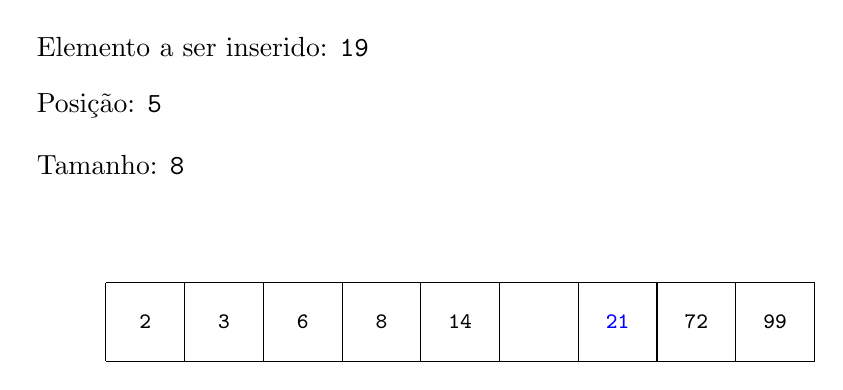
\begin{tikzpicture}
        \node[anchor=west] at (0, 4) {Elemento a ser inserido: \texttt{\textcolor{black}{19}}};
        \node[anchor=west] at (0, 3.25) {Posição: \texttt{\textcolor{black}{5}}};
        \node[anchor=west] at (0, 2.5) {Tamanho: \texttt{\textcolor{black}{8}}};
        \draw (1,0) grid (10,1);

        \node at (1.5,0.5) {\footnotesize \texttt{2}};
        \node at (2.5,0.5) {\footnotesize \texttt{3}};
        \node at (3.5,0.5) {\footnotesize \texttt{6}};
        \node at (4.5,0.5) {\footnotesize \texttt{8}};
        \node at (5.5,0.5) {\footnotesize \texttt{14}};
        \node at (6.5,0.5) {\footnotesize \texttt{}};
        \node at (7.5,0.5) {\footnotesize \texttt{\textcolor{blue}{21}}};
        \node at (8.5,0.5) {\footnotesize \texttt{\textcolor{black}{72}}};
        \node at (9.5,0.5) {\footnotesize \texttt{\textcolor{black}{99}}};
    \end{tikzpicture}

\end{frame}

\begin{frame}[fragile]{Visualização da inserção em posição arbitrária}

    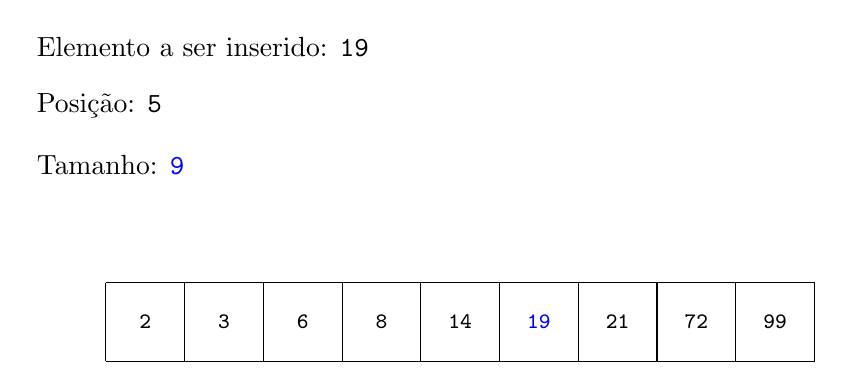
\begin{tikzpicture}
        \node[anchor=west] at (0, 4) {Elemento a ser inserido: \texttt{\textcolor{black}{19}}};
        \node[anchor=west] at (0, 3.25) {Posição: \texttt{\textcolor{black}{5}}};
        \node[anchor=west] at (0, 2.5) {Tamanho: \texttt{\textcolor{blue}{9}}};
        \draw (1,0) grid (10,1);

        \node at (1.5,0.5) {\footnotesize \texttt{2}};
        \node at (2.5,0.5) {\footnotesize \texttt{3}};
        \node at (3.5,0.5) {\footnotesize \texttt{6}};
        \node at (4.5,0.5) {\footnotesize \texttt{8}};
        \node at (5.5,0.5) {\footnotesize \texttt{14}};
        \node at (6.5,0.5) {\footnotesize \texttt{\textcolor{blue}{19}}};
        \node at (7.5,0.5) {\footnotesize \texttt{\textcolor{black}{21}}};
        \node at (8.5,0.5) {\footnotesize \texttt{\textcolor{black}{72}}};
        \node at (9.5,0.5) {\footnotesize \texttt{\textcolor{black}{99}}};
    \end{tikzpicture}

\end{frame}

\begin{frame}[fragile]{Implementação da função \rawcode{push()}}
    \inputsnippet{c}{86}{106}{vector_adt.c}
\end{frame}

\begin{frame}[fragile]{Exemplo de inserções}
    \inputsnippet{c}{1}{21}{passageiros.c}
\end{frame}

\begin{frame}[fragile]{Exemplo de inserções}
    \inputsnippet{c}{22}{41}{passageiros.c}
\end{frame}
